\documentclass{article}

\usepackage{fullpage}
\usepackage{titlesec}
\usepackage{parskip}
\usepackage{graphicx}
\usepackage{bold-extra}

\titleformat{\section}{\normalsize\bf}{\thesection \hspace{5pt}}{0em}{}
\titleformat{\subsection}{\normalsize\bf}{\thesubsection \hspace{5pt}}{0em}{}

\begin{document}

\centerline{\large{\textbf{Distributed Multi-Heuristic A* (HAMSTAR)}}}
\centerline{Noam Brown, Aram Ebtekar, Yuzuko Nakamura}
\centerline{15-712 Fall 2014 Final Project Report}

\section{Abstract}

A* is a popular graph search algorithm used in many artificial intelligence applications. The original A* algorithm makes use of a single heuristic to prioritize exploration through a graph, but a variation on the algorithm known as multi-heuristic A* (MHA*) makes use of multiple heuristics to more quickly arrive at approximate solutions. For this project we implemented a distributed version of MHA*, with one process per heuristic. We show... [performance]
%TODO: Highlight important results

\section{Introduction}

Weighted A* is a simple, heuristic-based search algorithm used in artificial intelligence applications such as robotics and games. A heuristic function estimates the remaining distance from any state to the goal, thus guiding the search toward the goal. If the heuristic is \textbf{admissible}, meaning it never overestimates the true distance, then the solution is guaranteed to be optimal to within the weight factor. If it meets a stronger condition called \textbf{admissibility}, then no state needs to be expanded more than once.

Finding good heuristic functions is difficult, and moreover, finding an admissible heuristic function that is reasonably accurate over the entirety of the search space is often not practical. Multi-heuristic A* (MHA*) \cite{Aine14} is an alteration of the A* algorithm that allows the usage of a combination of multiple arbitrary heuristics to guide the search, while retaining the optimality bound of wA* provided that one consistent heuristic is used as an �anchor�. Where the shortcomings of each individual heuristic may result in local optima which trap the search, the ability to change heuristics can provide an escape.

In their work, Aine et al. propose two variants on MHA*: Independent Multi-Heuristic A* (IMHA*), where path cost and shortest path information are tracked separately for each heuristic, and Shared Multi-Heuristic A* (SMHA*), where shared knowledge of path cost and shortest path information are updated by all heuristics. SMHA* is the more effective of the two (explores the graph in a less repetitive manner and enables more co-operation between heuristics), but is more difficult to parallelize due to the amount of shared data.

For this project, we implemented a distributed version of this second variant, SMHA*.

\section{Relevant Work}

Our work is directly based off of Aine et al.'s original multi-heuristic anchored search \cite{Aine14} mentioned above. A parallelized version of the original A* algorithm was presented by Phillips et al. \cite{phillips2014pa}. This method of parallelization makes inferences on when it's safe to expand multiple nodes in parallel, and in so doing maintains the approximate suboptimality guarantees of sequential wA*. This parallelization is dependent on the expansion operation being expensive enough to justify expanding multiple nodes in parallel, which may not be the case for all problems. By contrast, our method parallelizes the search process by constantly expanding multiple nodes chosen by different heuristics (instead of multiple nodes chosen by a single heuristic). As a result, our method differs from the previous in that, although nodes may be expanded multiple times by different machines, we do not require expansions to be slow.

\section{System Description}

\begin{figure}
\centering 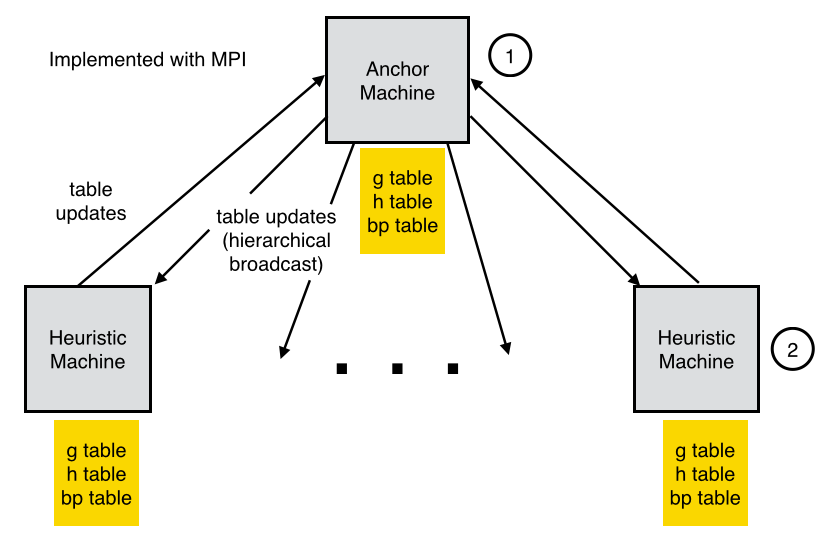
\includegraphics[width=5.0in]{system-diagram}
\caption{A diagram of our system. One machine starts up the others and runs the admissible anchor search. The other machines run their individual heuristics. Communication is done using MPI. 
\textcircled{1}\textbf{Anchor:} Starts heuristic machines; performs state expansions using anchor heuristic; receives, resolves, and broadcasts table updates; checks for termination conditions. \textcircled{2}\textbf{Heuristic:} Expands a likely state (chosen using heuristic); updates path cost to its successors; communicates updates to anchor; checks for termination conditions}
\label{fig:sysdiag}
\end{figure}

An overview of our system is in Figure \ref{fig:sysdiag}. The main (anchor) machine starts up other heuristic machines. Each machine runs its own heuristic, with the anchor machine's being the admissible heuristic. Each of the non-anchor heuristic machines periodically send updates of the data structures (tables containing shortest path information found so far) to the anchor machine, which compares the data it receives and sends out table updates of the best paths known so far to all other nodes.

\begin{figure}
\centering 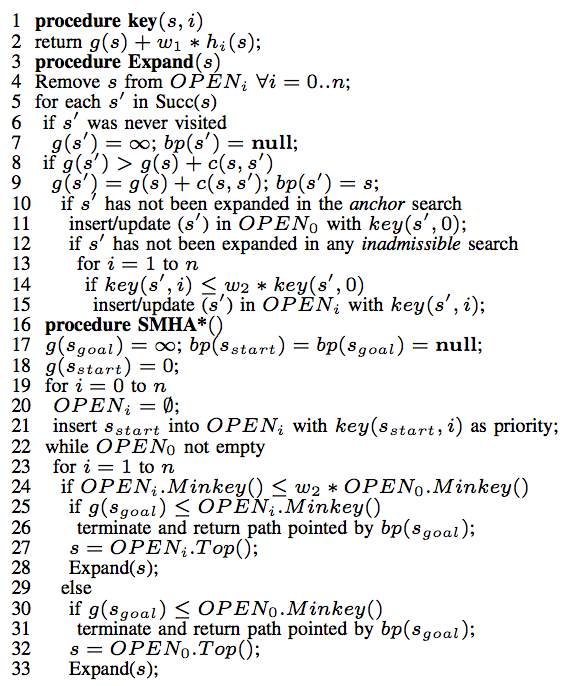
\includegraphics[width=3in]{pseudocode}
\caption{Pseudocode from Aine et al., detailing the original single-threaded version of the algorithm we parallelized.}
\label{fig:pseudocode}
\end{figure}


Our algorithm is based off of the single-threaded, round-robin SMHA* code presented in \cite{Aine14} (Figure \ref{fig:pseudocode}). Our parallelized code was written in C++ with inter-process communication accomplished using MPI. The work was distributed over one or more of the 16-core machines in the Apt cluster. % TODO: Machine specs here? Or in the experimental setup section?

\subsection{Design Decisions}

\textbf{Interprocess communication with MPI}

We investigated other frameworks designed for iterative algorithms on a stable dataset such as Spark and GraphLab. However, most of these frameworks were designed for chunking up a large dataset upon which a single operation is performed. Our application's needs differed from this model in that the dataset being operated on (the graph being explored) was shared by all workers, and the workers themselves were performing differing operations on subsets of the same data.

In the case where the working set of data is small enough to be contained within each process, the system is much less complex, and the services provided by Spark and GraphLab are not so crucial. For these reasons we instead decided to distribute our code using MPI.

\textbf{Synchronous broadcast vs. asynchronous sync-ups}

% TODO: Fill me in! MPI-specific feature...

\textbf{Update collation performed at anchor node}

In our system, updates are sent from heuristic machines to the anchor machine, which collects these updates and combines them into a smaller set of table updates. For example, if two heuristic machines both send new shortest path values for the same state, the anchor machine receives both and at a later time sends out an update on the shortest path to that state that is the minimum of values it received. All nodes then update their data structures with this new information. 
% TODO: ^ Is this right?

One alternative to this method of communicating updates would be to have each node periodically broadcast its table updates to all other nodes and each node would incorporate those updates in its own table. This requires many more messages to go over the network and work to be duplicated. However, in the case where the anchor node is overloaded or has a possibility of going down, this alternative would be more appealing. We didn't consider this to be within the scope of this project, however, so we only implemented a system of update collation at the anchor machine. However, this may be interesting to investigate in the future.
%TODO: Maybe justfiy or link with any result that indicates that the anchor node's workload becomes a bottleneck (or doesn't)




\section{Experimental Setup}

We tested our algorithm on a set of four random sliding tile puzzles of size 5x5, averaging the results of each trial into a single result. The data we collected were (1) running time, (2) number of states in the problem graph that were expanded during the course of searching for a solution, and (3) the length in steps of the best solution at termination.

%TODO: ^ Explain how the states expanded node is calculated? Maybe as a footnote?

% TODO: Apt? Machine specs?

% TODO: Talk about what we varied for the tests. Frequency of communication, effect of adding more heuristics, effect of adding more machines (maybe we want a graph that compares the effect of adding more heuristics on the same machine vs. adding more heuristics by using more machines), and comparison to single thread/round robing running time

In MHA*, two weights are specified. The first weight ($w_1$) determines how much priority to give heuristic expansions over the anchor search. A higher $w_1$ results in more depth-first-search-like behavior. The second weight ($w_2$) determines how close to the current known minimum path length a path to the goal must be before being selected as a solution. MHA* gives a guarantee that the solution found at termination is at most $w_1 * w_2$ times the optimum value. For all experiments, we used $w_1$, $w_2 = 2$. Note that when there is only one heuristic in a test (the admissible heuristic), the optimal shortest path to the goal will be found by only having to expand each state at most once (guaranteed by running A* with an admissible heuristic) and neither $w_1$ nor $w_2$ have any effect.

\section{Results}

% TODO: I need to put a ton of graphs and tables here


\section{Conclusions}

% TODO: Fill me in!



% TODO: Should we have some kind of discussion on whether the parallelized version of SMHA* keeps the w1*w2 optimality guarantees that the single-threaded version does?? Also, maybe part of this, but the longer we go without doing a table update sync-up, the more the algorithm resembles IMHA*. It might be good to point this out somewhere, maybe in the Results/Discussion section




%\section{Final Paper Outline}

%\subsection{Introduction}
%\subsection{Related Work}
%\subsection{System Description}
%\subsection{Evaluation}
%\subsection{Conclusions and Future Work}

\bibliographystyle{ieeetr}
\bibliography{sources}


\end{document}